%use in documents with \subfile{tex/intro}
\documentclass[../../master.tex]{subfiles}

\begin{document}

\section{The \textit{Azoarcus} Group I Intron}
\label{sec:theory:gii}

A large class of ribozymes are the so-called group I introns. 
These catalytically active RNA molecules are common in a large variety of genomes, being found in bacteria, eukaryotes, organelles, even in archaea and viruses \parencite{zhou_gissd_2008, nawrocki_group_2018}.
Although being very variable in primary sequence composition and length, defining characteristics of these ribozymes are high conservation of their secondary structure and a shared primary catalytic function; self-splicing from the precursor RNAs they are embedded in \parencite{zhou_gissd_2008}.


The bacterium \textit{Azoarcus sp. BH72} contains a group I intron located in the precursor of its Isoleucine codon-binding tRNA (pre-tRNA\textsuperscript{Ile}), which is compelling for multiple reasons.
With a sequence length of around 200 nucleotides, it is a particularly small group I intron. 
It has been shown to retain its catalytic activity at high temperatures up to \unit[80]{\textdegree C} \parencite{tanner_activity_1996}.
Furthermore, its outstanding capability of self-assembly (see \autoref{sub:theory:azoarcus_selfassembly} for details) from smaller fragments piques interest in the context of the RNA world hypothesis. 

\subsection{Structural Features}
\label{sub:theory:azoarcus_structurefeatures}

Since RNA function is in large parts influenced by structure, taking a closer look at its structure beforehand is valuable in understanding the function of the \textit{Azoarcus} group I intron.
Not less importantly, some details of the ribozymes structure should be considered to increase the likelihood of successful RNA sequence design.

The conserved catalytic core of group I introns consists of two structural domains, P4-P6 and P3-P9, of which the latter only contains the helices P3, P7, P8 and P9 \parencite{tanner_joining_1997}. 
These domains are displayed as a secondary structure in \autoref{fig:azostructure}.

\begin{figure}[!ht]
	\centering
	%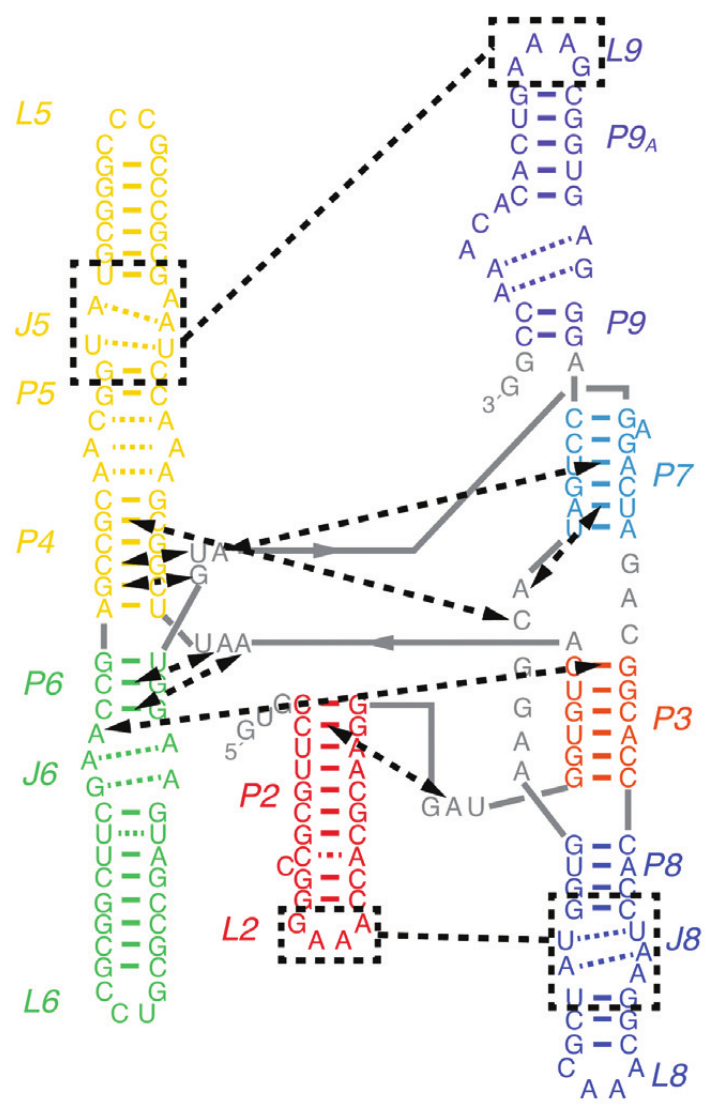
\includegraphics[width=0.45\textwidth]{pic/intro/azoarcus/mustoe2016_fig1a.png}
	\begin{tikzpicture}
		\node[anchor=south west] (image) at (0,0) {
			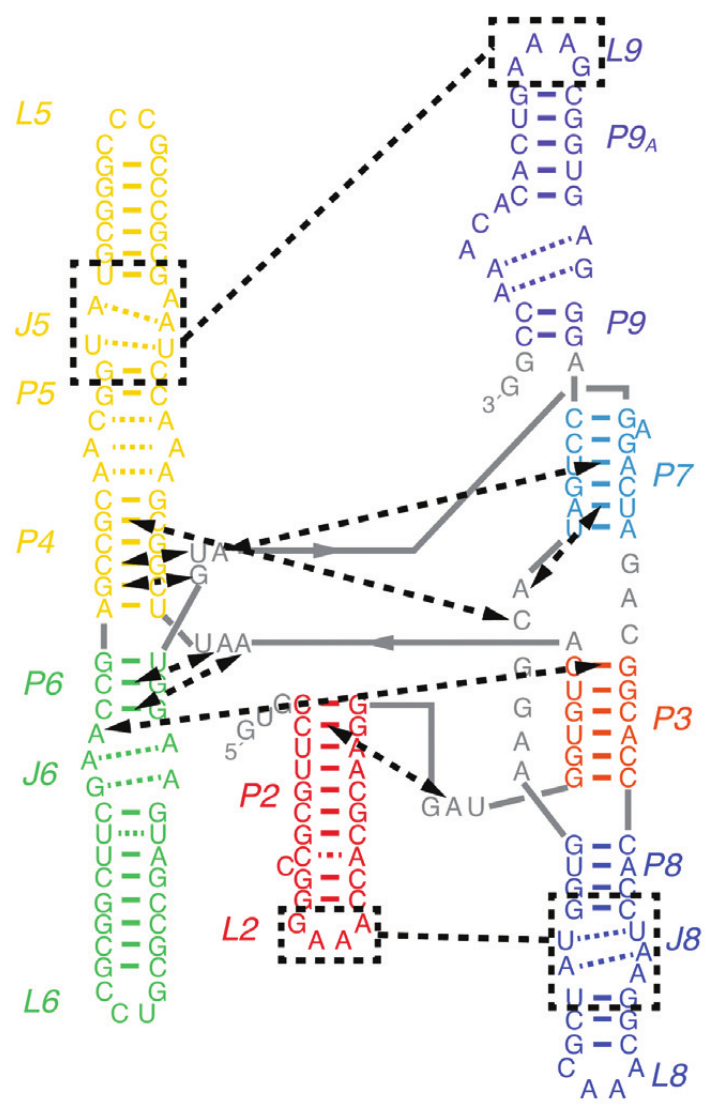
\includegraphics[width=0.45\textwidth]{pic/intro/azoarcus/mustoe2016_fig1a.png}
		};
		\node[anchor=west] (bulge) at (6.2,6.55) {\footnotesize \} \unit[1]{nt} bulge};
	\end{tikzpicture}
	
	\caption[Secondary Structure of the \textit{Azoarcus} Group I Intron]{Secondary structure of the \textit{Azoarcus} Group I Intron. Dashed black lines indicate long-range tertiary interactions, and colored dashed lines indicate noncanonical base pairs. Note that P3 and P7 form a pseudoknot and that P7 contains a single-nucleotide bulge. This secondary structure corresponds to \texttt{PDB 1U6B} \parencite{adams_crystal_2004}. Modified after \parencite[Figure 1A]{mustoe_secondary_2016}.
	}\label{fig:azostructure}
\end{figure}


The presence of the (scaffold) domain P4-P6 is not strictly required to retain the catalytic function of the intron, albeit removal reduces the efficiency of the catalytic domain \parencite{hayden_intramolecular_2015}.
Yet, crucial components of the \textit{Azoarcus} group I intron structure are, in fact, part of its tertiary structure; the helices P3 and P7 form an H-type pseudoknot.
This pseudoknot is of importance as P7 contains the guanosine binding site required for the introns self-splicing activity (see \autoref{sub:theory:azoarcus_selfsplicing}) \parencite{kuo_characterization_1999}.
This binding site is in direct proximity of the \unit[1]{nt} bulge in P7 as is often the case for recognition and binding motifs \parencite{turner_bulges_1992, hermann_rna_2000}.
Additionally, the nucleotide identities in P7 are highly conserved among group I introns \parencite{zhou_gissd_2008}.
In other group I introns, it has been shown that tertiary interactions contribute to the formation of the catalytic core \parencite{tanner_joining_1997}.
The tertiary interactions in \texttt{Azoarcus} are relatively non-specific with respect to the sequence but largely determined by its native secondary structure \parencite{mustoe_secondary_2016} (\autoref{fig:azostructure}).

\subsection{Self-Splicing}
\label{sub:theory:azoarcus_selfsplicing}

Self-splicing in \textit{Azoarcus} follows the same two-step mechanism as seen in other group I introns \parencite{gleitsman_kinetic_2014}.
The first step  is initiated by exogenous guanosine monophosphate ($\alpha\mathrm{G}$) binding at the active site of the intron (\emph{pre-1S}) followed by an attack of the $\alpha\mathrm{G}$ 3'-hydroxy group on the phosphodiester bond at the 5'-exon splice site (\emph{post-1S}, see \autoref{fig:selfsplicing}) \parencite{adams_crystal_2004-1, gleitsman_kinetic_2014}.
It is now phosphorylated at the 5' end of the intron.

\begin{figure}[!ht]
	\centering
	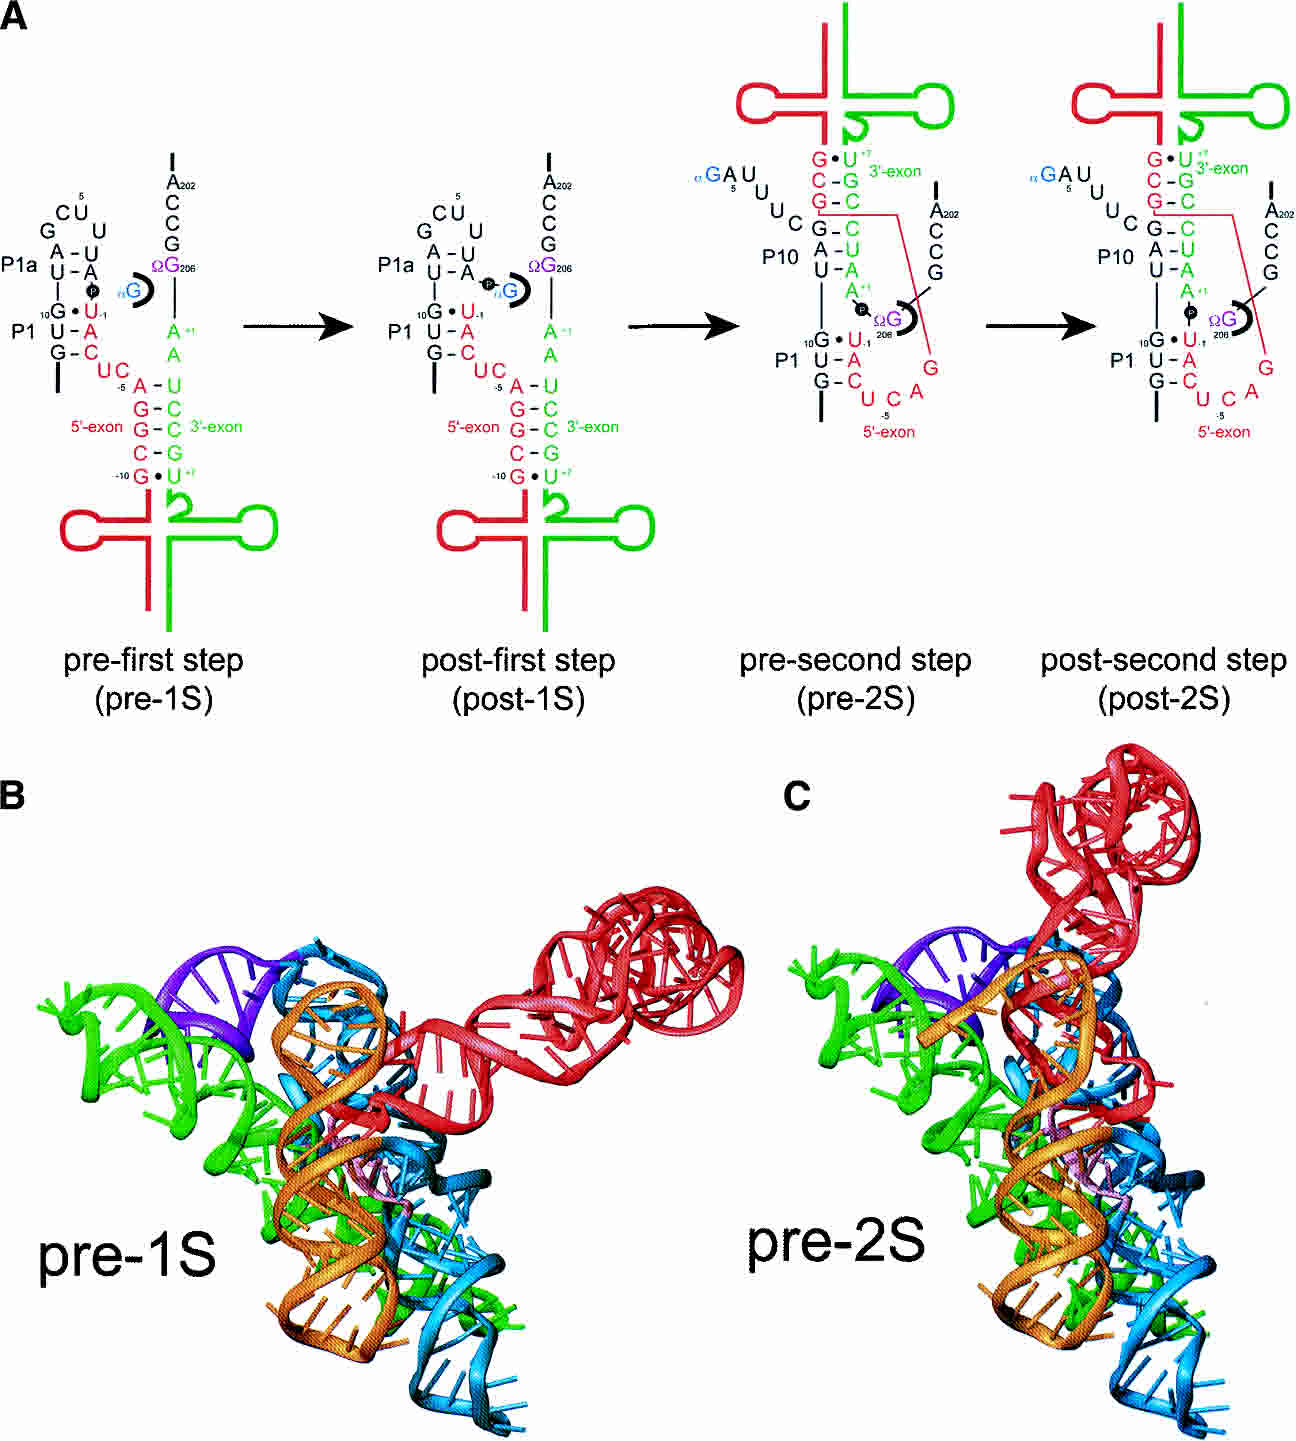
\includegraphics[trim=0 700 0 30, clip, width=0.8\textwidth]{pic/intro/notmine/adams2004-1_fig19A.png}
	\caption[Self-Splicing of the \textit{Azoarcus} Group I Intron]{
		Overview of the self-splicing reaction. 
		The guanosine binding site is stylized as a black pocket.
		Splice sites are marked as bold dots on backbone bonds.
		The change of orientation of the exons in \emph{pre-2S} and \emph{post-2S} indicates the conformational change of the ribozyme during self-splicing.
		Taken from \parencite[Figure 19A]{adams_crystal_2004-1}.
	}\label{fig:selfsplicing}
\end{figure}


Following a conformational change of the intron, the second step results in splicing both exons; the 3'terminal G ($\Omega\mathrm{G}$) of the intron binds to the binding site (\emph{pre-2S}), which allows the hydroxy group now attached at the 5'-exon to attack the phosphodiester bond.
This enables a transfer of the hydroxy group to $\Omega\mathrm{G}$ and immediate ligation of both exons (\emph{post-2S}) \parencite{adams_crystal_2004-1}. 
This two-step transesterification requires proximity between both splicing sites and the guanosine binding site, which is maintained after the first step by binding the 5'-exon to the internal guide sequence (IGS).

This mechanism is not limited to self-splicing of the intron; spliced-out ribozymes catalyze cleavage and ligation of oligonucleotides resembling the 5'-exon \parencite{kuo_characterization_1999, gleitsman_kinetic_2014}.
A related reaction scheme is later described in \autoref{ssub:exp_results:assay}.

\subsection{Self-Assembly}
\label{sub:theory:azoarcus_selfassembly}

Building on the primary self-splicing activity characteristic for group I introns, the \textit{Azoarcus} group I intron has been shown to catalyze self-assembly from smaller inactive fragments by \citeauthor{hayden_self-assembly_2006} \parencite{hayden_self-assembly_2006}, making it a promising candidate to support the RNA world hypothesis.

Similar to its self-splicing reaction mechanism via a two-step transesterification, the \textit{Azoarcus} group I intron can catalyze the recombination and ligation of RNA sequences where a trinucleotide \texttt{CAU} complementary to the IGS is accessible as the recognition motif \parencite{hayden_rna-directed_2005}.

Leveraging this mechanism, \citeauthor{hayden_self-assembly_2006} placed \texttt{CAU} trinucleotides into the L5, L6 and L8 hairpin loop regions of the intron, which then was split into four inactive fragments \parencite{hayden_self-assembly_2006}.
Incubation of the inactive fragments leads to (non-covalent) \textit{trans}-assembly of a functional RNA complex catalyzing ligation of the incubated fragments by recombination (\autoref{fig:selfassembly}) \parencite{hayden_self-assembly_2006, hayden_systems_2008}.

\begin{figure}[!ht]
	\centering
	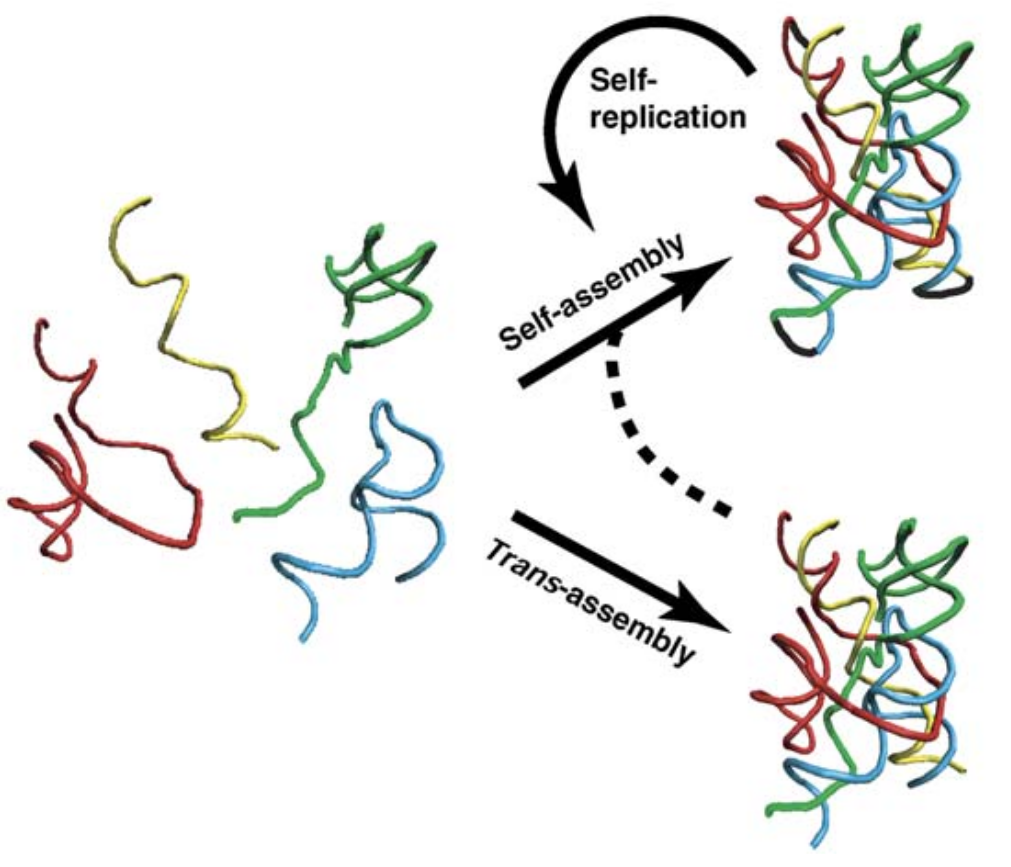
\includegraphics[width=0.6\textwidth]{pic/intro/notmine/hayden2006_figure2B.png}
	\caption[Self-Assembly of the \textit{Azoarcus} Group I Intron]{
		Formation of a \textit{trans}-complex from inactive fragments catalyzes covalent assembly of the \textit{Azoarcus} ribozyme which then in turn facilitates self-assembly.
		Taken from \parencite[Figure 2B]{hayden_self-assembly_2006}.
	}\label{fig:selfassembly}
\end{figure}

Due to its autocatalytic replication capabilities, the \textit{Azoarcus} group I intron is a vital model system supporting the RNA world hypothesis.
Even more so, by modifying the IGS and the corresponding recognition motifs, cooperative replicator networks can be constructed.
Specifically, \citeauthor{vaidya_spontaneous_2012} partitioned the \textit{Azoarcus} ribozyme into two fragments instead of four by selecting a single site of the three loops used by \citeauthor{hayden_self-assembly_2006} \parencite{vaidya_spontaneous_2012}.
Because of the three loops, this yielded three distinct fragment pairs assembling into the same ribozyme.
The recognition motif of each fragment pair was modified to be unique with respect to the other two. 
Replacing the IGS of each fragmented ribozyme matching to the recognition motif of one of the others lead to a network of three catalysts, cooperatively assembling each other like in a biomolecular game of \emph{rock-paper-scissors}.



\end{document}
